%\section{KAPITEL}
%\subsection{TITLE}
%\frame {
%    \frametitle{TITLE}
%    \begin{itemize}
%    \item
%    \end{itemize}
%}


\section{Intro}
\subsection{whoami}
\frame {
    \frametitle{Johannes Raggam}
    \begin{itemize}
    \item Graz, Österreich
    \item Web-Entwicklung seit 2002
    \item Plone Entwicklung seit 2005
    \item Deliverance User seit 2009
    \item Mitglied der BlueDynamics Alliance
    \item Web: \url{http://johannes.raggam.co.at/}
    \end{itemize}
}

% BEGIN BSP1-1
\subsection{Beispiel}
\frame {
    \begin{columns}[t]
        \begin{column}{6.5cm}
            {\small\textbf{Content}}\\
            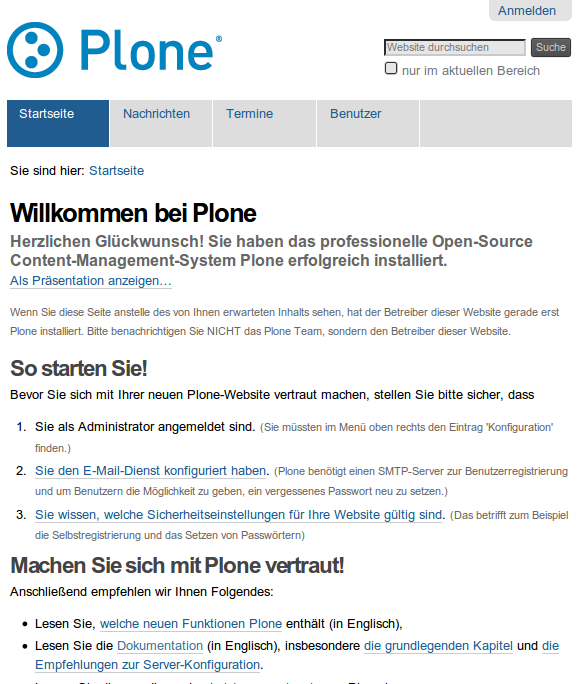
\includegraphics[scale=0.31]{resources/bsp1-plone-plain}
        \end{column}
        \begin{column}{6.5cm}
            {\small\textbf{Theme}}\\
            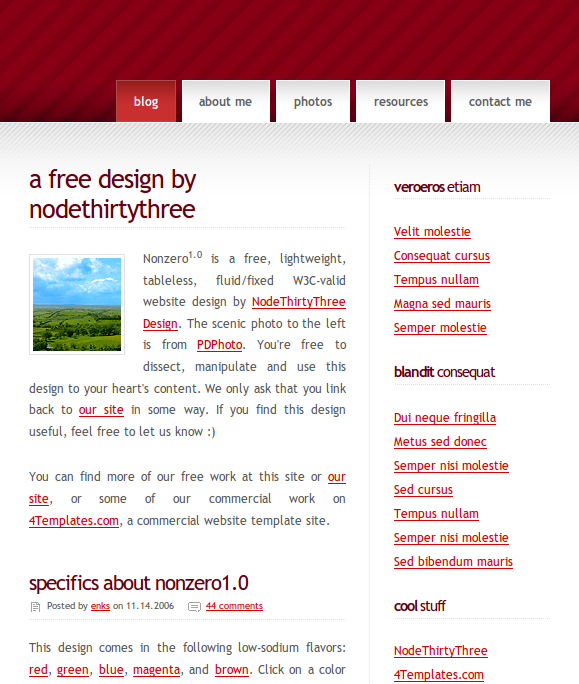
\includegraphics[scale=0.31]{resources/bsp1-nonzero-plain}
        \end{column}
    \end{columns}
}

\frame {
    \begin{columns}[t]
        \begin{column}{6.5cm}
            {\small\textbf{Content}}\\
            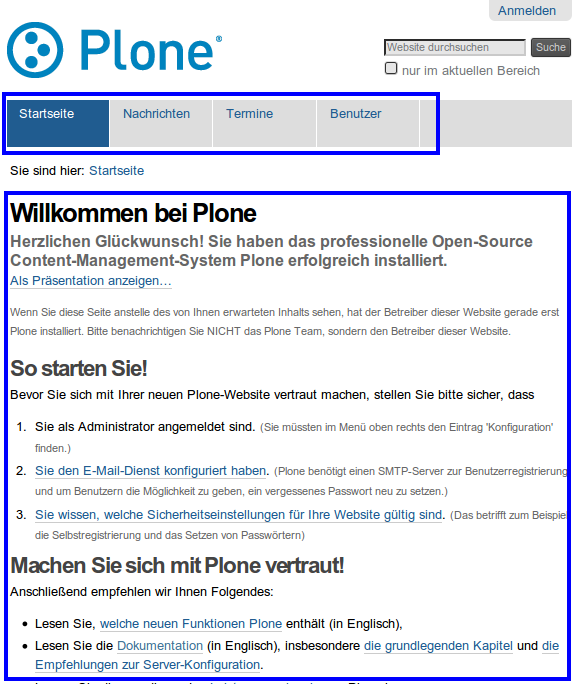
\includegraphics[scale=0.31]{resources/bsp1-plone-plain-h}
        \end{column}
        \begin{column}{6.5cm}
            {\small\textbf{Theme}}\\
            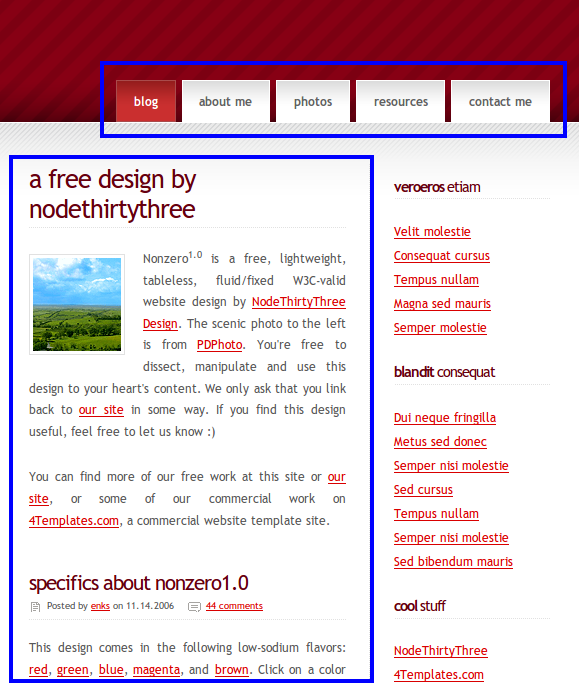
\includegraphics[scale=0.31]{resources/bsp1-nonzero-plain-h}
        \end{column}
    \end{columns}
}

\frame {
    \begin{columns}[t]
        \begin{column}{6.5cm}
            {\small\textbf{Content}}\\
            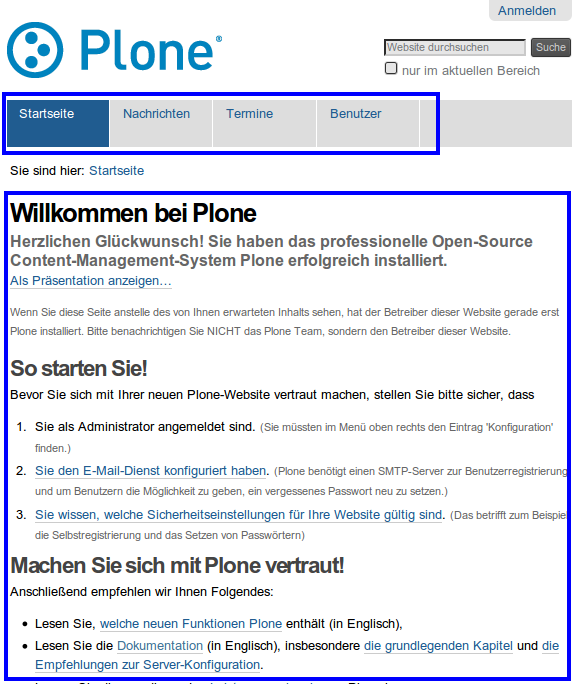
\includegraphics[scale=0.31]{resources/bsp1-plone-plain-h}
        \end{column}
        \begin{column}{6.5cm}
            {\small\textbf{Theme}}\\
            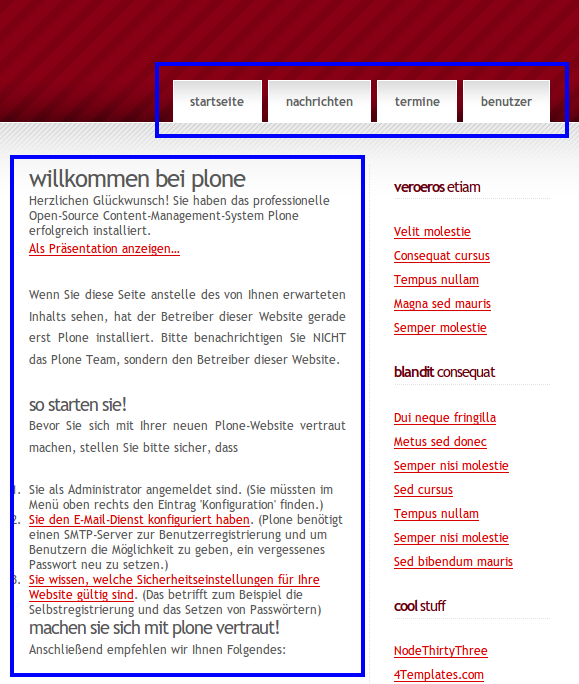
\includegraphics[scale=0.31]{resources/bsp1-nonzero-plone-h}
        \end{column}
    \end{columns}
}

\frame {
    \begin{columns}[t]
        \begin{column}{6.5cm}
            {\small\textbf{Content}}\\
            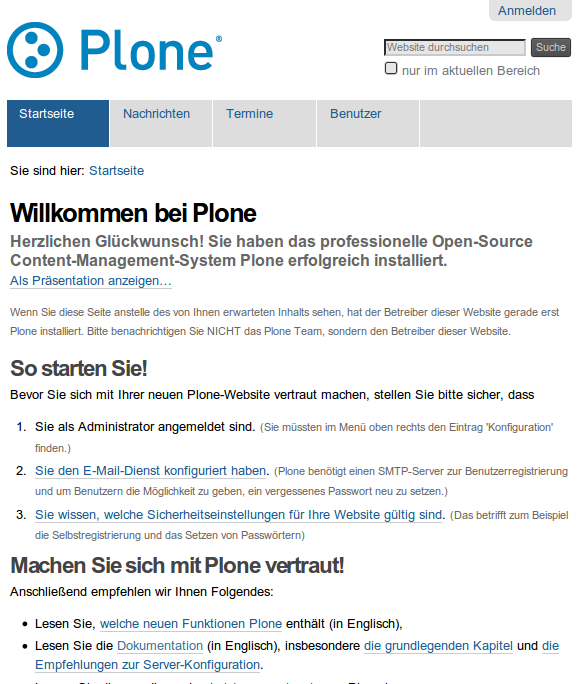
\includegraphics[scale=0.23]{resources/bsp1-plone-plain}
        \end{column}
        \begin{column}{6.5cm}
            {\small\textbf{Theme}}\\
            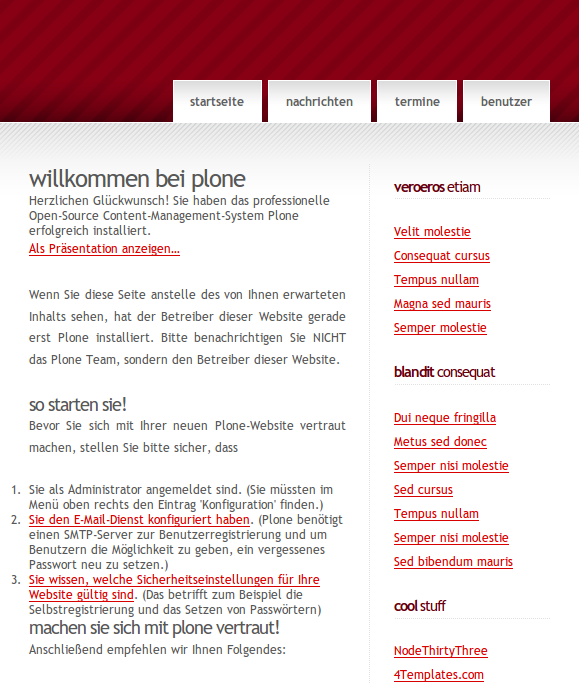
\includegraphics[scale=0.23]{resources/bsp1-nonzero-plone}
        \end{column}
    \end{columns}
    \begin{columns}[t]
        \begin{column}{12cm}
{\scriptsize\texttt{
$<$replace content="\#portal-globalnav" theme="children:\#menu" $/>$\\
$<$replace content="children:\#content" theme="children:\#columnA\_2columns" $/>$
}}
        \end{column}
    \end{columns}
}
% END BSP1-1

% BEGIN BSP1-2
\frame {
    \begin{columns}[t]
        \begin{column}{6.5cm}
            {\small\textbf{Content}}\\
            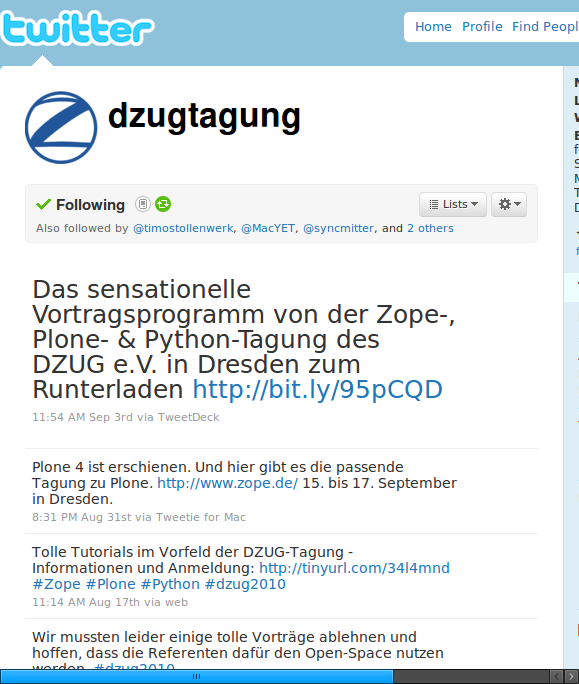
\includegraphics[scale=0.31]{resources/bsp1-twitter-plain}
        \end{column}
        \begin{column}{6.5cm}
            {\small\textbf{Theme}}\\
            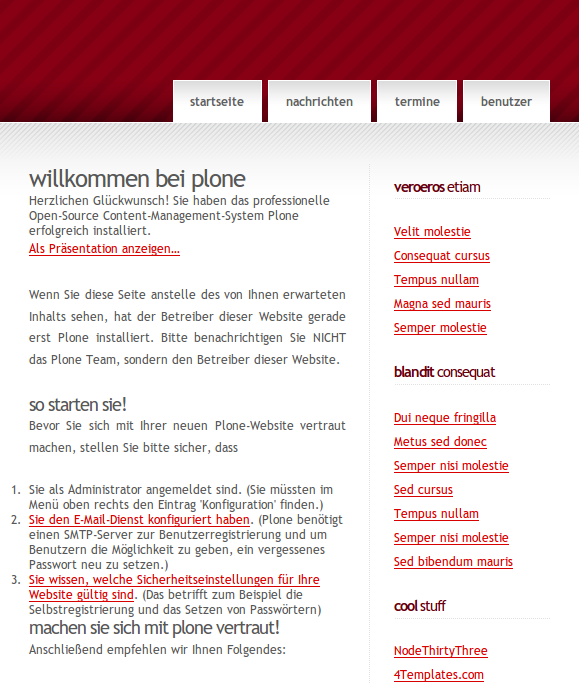
\includegraphics[scale=0.31]{resources/bsp1-nonzero-plone}
        \end{column}
    \end{columns}
}

\frame {
    \begin{columns}[t]
        \begin{column}{6.5cm}
            {\small\textbf{Content}}\\
            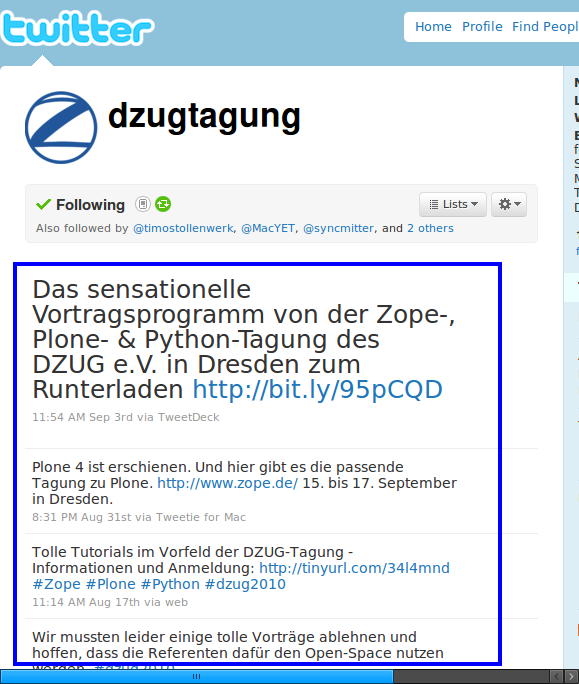
\includegraphics[scale=0.31]{resources/bsp1-twitter-plain-h}
        \end{column}
        \begin{column}{6.5cm}
            {\small\textbf{Theme}}\\
            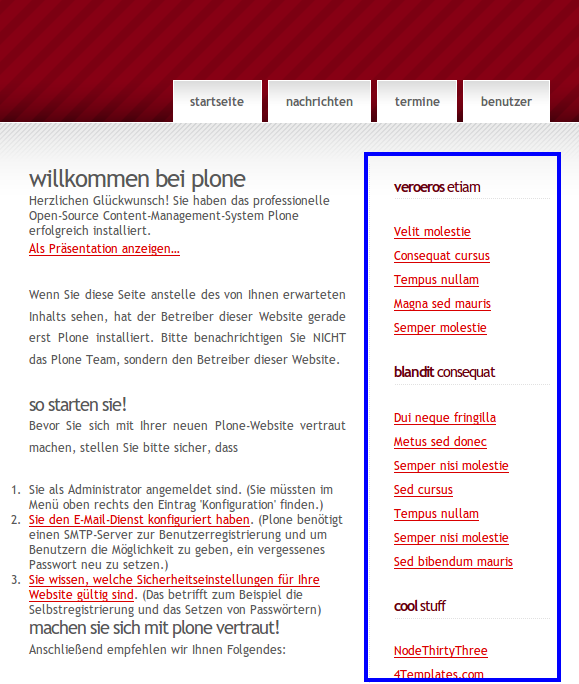
\includegraphics[scale=0.31]{resources/bsp1-nonzero-plone-h2}
        \end{column}
    \end{columns}
}

\frame {
    \begin{columns}[t]
        \begin{column}{6.5cm}
            {\small\textbf{Content}}\\
            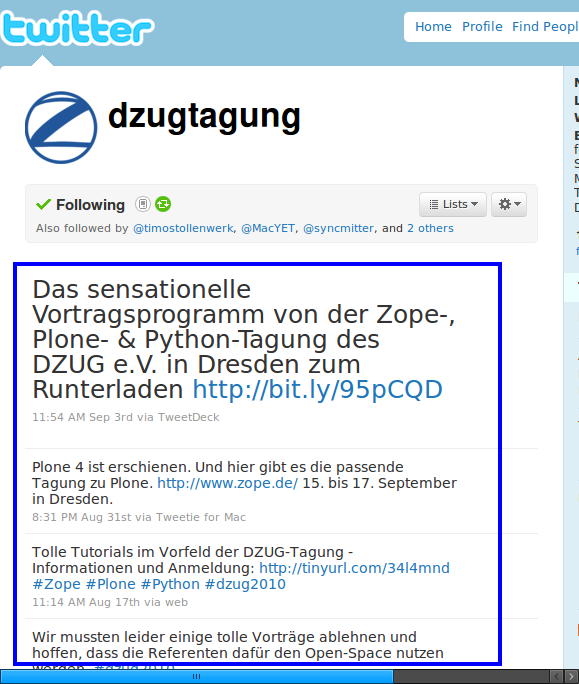
\includegraphics[scale=0.31]{resources/bsp1-twitter-plain-h}
        \end{column}
        \begin{column}{6.5cm}
            {\small\textbf{Theme}}\\
            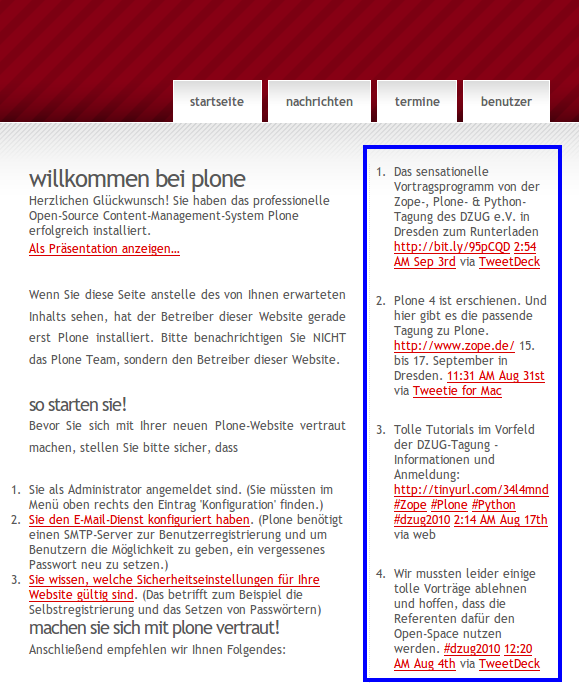
\includegraphics[scale=0.31]{resources/bsp1-nonzero-plone-twitter-h}
        \end{column}
    \end{columns}

}

\frame {
    \begin{columns}[t]
        \begin{column}{6.5cm}
            {\small\textbf{Content}}\\
            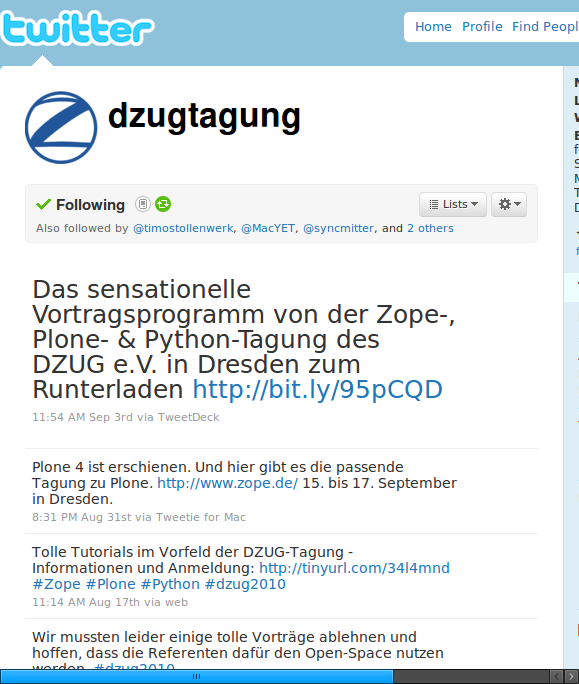
\includegraphics[scale=0.23]{resources/bsp1-twitter-plain}
        \end{column}
        \begin{column}{6.5cm}
            {\small\textbf{Theme}}\\
            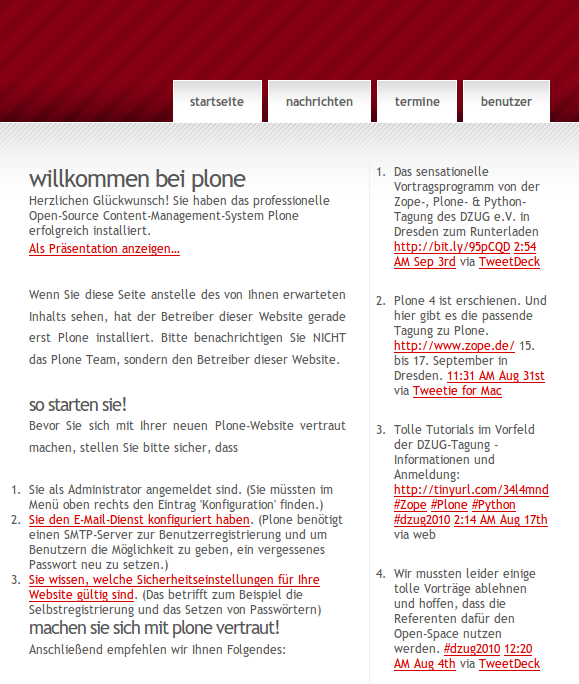
\includegraphics[scale=0.23]{resources/bsp1-nonzero-plone-twitter}
        \end{column}
    \end{columns}
    \begin{columns}[t]
        \begin{column}{12cm}
{\scriptsize\texttt{
$<$replace href="http://twitter.com/dzugtagung"\\
         content="\#timeline" theme="children:\#columnC\_2columns"$/>$
}}
        \end{column}
    \end{columns}
}
% END BSP1-2



\section{Hintergrund}
\subsection{Problemfeld}
\frame {
    \vfill
    \center{
    \huge\textbf{Webdesign = essentiell}\\
    \huge\textbf{Design Integration = mühsam}
    }
    \vfill
}

\subsection{Designprozess aktuell}
\frame {
    \frametitle{Designprozess aktuell}
    \begin{itemize}
    \item Unterschiedliche Plattformen - Unterschiedliche Techniken
        \begin{itemize}
            \item Plone, Django, Drupal, Wordpress, Joomla, ...
        \end{itemize}
    \item Umfangreiches Wissen notwendig
        \begin{itemize}
            \item HTML, CSS, JS
            \item CMS Interna: Templatemechanismus, Konfiguration, Integration
            \item Deploymentprozess
        \end{itemize}
    \end{itemize}
}

\subsection{Designprozess aktuell - Workflow}
\frame {
    \frametitle{Designprozess aktuell - Workflow}
    \begin{itemize}
        \item Designteam
            \begin{itemize}
                \item Erstellung HTML Template
            \end{itemize}

        \item Entwicklungsteam
            \begin{itemize}
                \item Integration in Zielsystem
                \item Veröffentlichung
            \end{itemize}

        \item Designänderungen kommen bestimmt
            \begin{itemize}
                \item Wasserfallmodell: Änderungen in nachfolgenden Phasen aufwändig
                \item Enge Kopplung Designteam - Entwicklungsteam
            \end{itemize}

    \end{itemize}
}

\subsection{Lösung? Deliverance. XDV.}
\frame {
    \frametitle{Workflow mit Deliverance}
    \begin{itemize}
    \item Designteam
        \begin{itemize}
        \item HTML Theme, CSS, JS
        \item eventuell rules.xml
        \item Ideal: selbstständiges Deployment
        \end{itemize}
    \item Entwicklungsteam
        \begin{itemize}
        \item Kleinteilige Layoutarbeiten
        \item rules.xml
        \end{itemize}
    \end{itemize}
}


\subsection{Entwicklungsgeschichte}
\frame {
    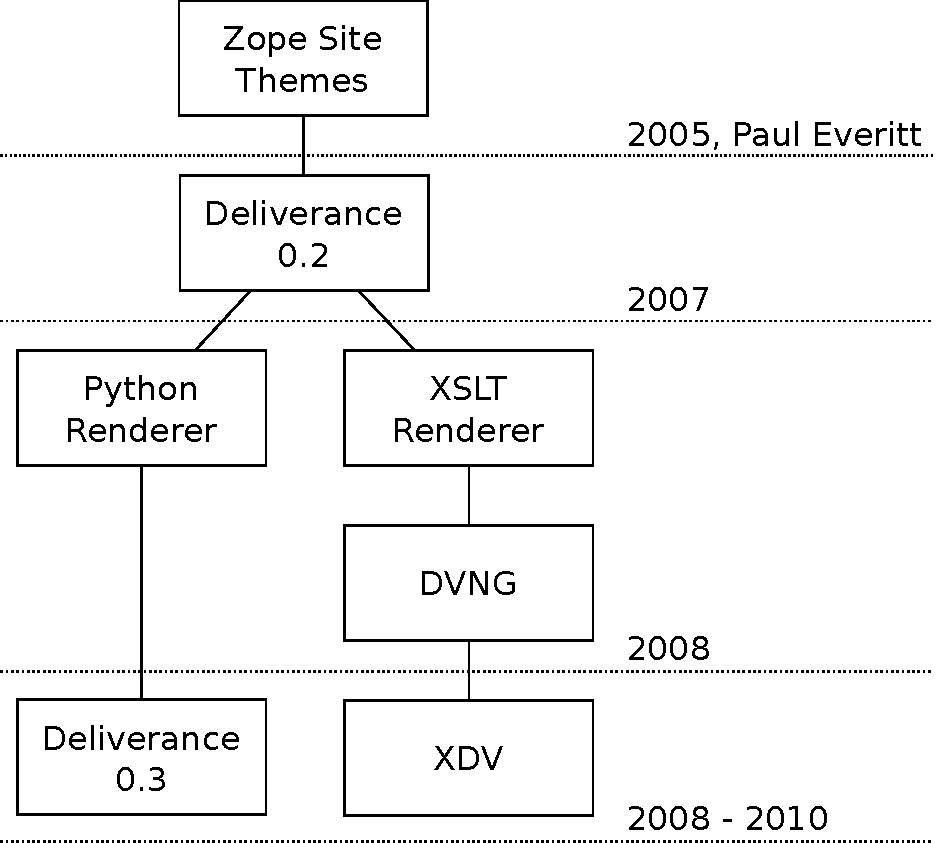
\includegraphics[scale=0.4]{resources/deliverance-xdv-history-wtext}
}



%\subsection{Funktionsweise}
%\frame {
%    % TODO: graphik mit rules übersicht
%}



\section{Deliverance}

\subsection{Was ist Deliverance?}
\frame {
    \frametitle{Was ist Deliverance?}
    \begin{itemize}
    \item Theming Engine für unterschiedliche Plattformen
        \begin{itemize}
        \item Einheitliches Layout fürverschiedene Applikationen (bsp Plone und Wordpress)
        \item Einfache Mashups: Inhalte können durch \texttt{href} Attribut referenziert werden.
        \end{itemize}
    \item HTML Transformation durch Mapping von Elementen
    \item Trennung Präsentation - Inhalt
        \begin{itemize}
        \item Verbesserter Workflow Designteam - Entwicklerteam
        \end{itemize}
    \end{itemize}
}

\subsection{Regeln}
\frame {
    \frametitle{Deliverance Regeln}
    \begin{itemize}
        \item \textbf{drop}: {\small{Entfernt Element aus Content oder Theme}}\\
        {\scriptsize\texttt{$<$drop content="SELEKTOR" $/>$, $<$drop theme="SELEKTOR" $/>$}}

        \item \textbf{replace}: {\small{Ersetzt Element in Theme durch Content}}\\
        {\scriptsize\texttt{$<$replace content="SELEKTOR" theme="SELEKTOR" $/>$}}
        \item \textbf{append}: {\small{Fügt Element in Theme durch Content am Ende hinzu}}\\
        {\scriptsize\texttt{$<$append content="SELEKTOR" theme="SELEKTOR" $/>$}}
        \item \textbf{prepend}: {\small{Fügt Element aus Content in Theme am Anfang hinzu}}
        {\scriptsize\texttt{$<$prepend content="SELEKTOR" theme="SELEKTOR" $/>$}}
    \end{itemize}
}

\subsection{Selektoren}
\frame {
    \frametitle{Deliverance Selektoren}
    \begin{itemize}
    \item CSS 3 Selektoren
        \begin{itemize}
        \item \#content, .header, div[href='.kss']
        \end{itemize}
    \item XPATH Selektoren
        \begin{itemize}
        \item /html/head/title
        \item /html/body/div[1]/a[3]
        \end{itemize}
    \item Selektor Typen
        \begin{description}
        \item[element] (default) Gesamtes Element
        \item[children] Kindelemente
        \item[tag] Element ohne Kindelemente
        \item[attribute] Attribute des ausgewählten Elements
        \item[Beispiel] \texttt{content="children:\#maintext"}\\
        \texttt{content="attribute(class):body"}
        \end{description}
    \end{itemize}
}

\subsection{Systemskizze}
\frame {
    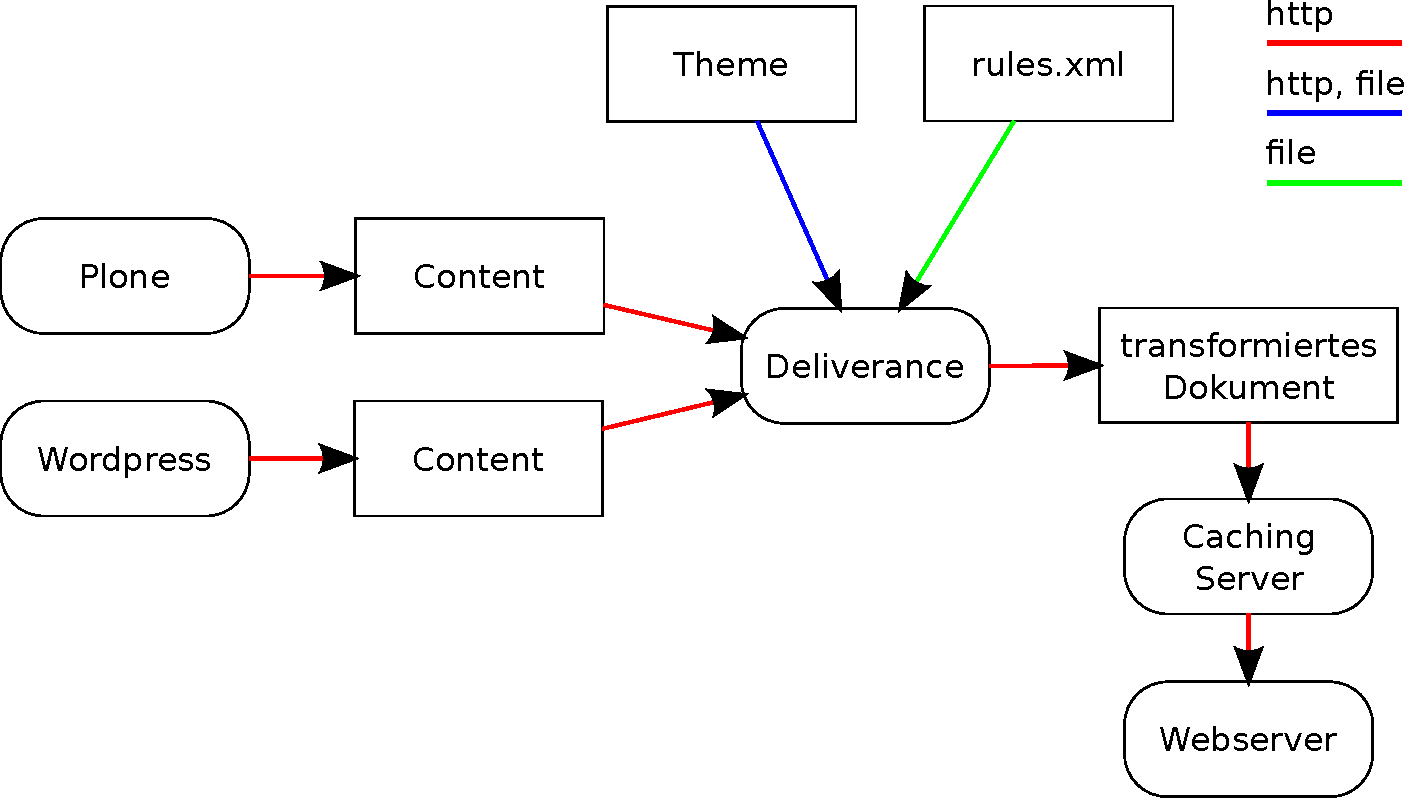
\includegraphics[scale=0.4]{resources/deliverance-systemskizze}
}


\section{XDV}
\subsection{Allgemein}
\frame {
    \frametitle{Allgemein}
    \begin{itemize}
    \item XSLT basiert
        \begin{itemize}
        \item Inline XSL
        \item Mehr Deployment-Optionen
        \item Schneller (ca 10ms statt 30ms Overhead)
        \end{itemize}
    \item Selektoren
        \begin{itemize}
        \item XPATH (default)
        \item CSS3 (via css:theme="" )
        \end{itemize}
    \item Keine Selektortypen
    \item Keine Debug Konsole
    \end{itemize}
}

\subsection{Regeln}
\frame {
    \frametitle{XDV Syntax: Deliverance 0.2 Syntax + Erweiterungen}
    \begin{tabular}{ll}
    \textbf{XDV} & \textbf{Deliverance}\\
    \hline
    \texttt{replace} & \texttt{replace}\\
    \texttt{copy} & \texttt{replace} + \texttt{children} Selektortyp\\
    \texttt{before} & \texttt{prepend}\\
    \texttt{after} & \texttt{append}\\
    \texttt{prepend} & \texttt{prepend} + \texttt{children} Selektortyp\\
    \texttt{prepend} + XPATH @ & \texttt{prepend} + \texttt{attribute} Selektortyp\\
    \texttt{append} & \texttt{append} + \texttt{children} Selektortyp\\
    \texttt{drop} & \texttt{drop}\\
%        \texttt{}
    \end{tabular}
}

\subsection{Systemskizze}
\frame {
    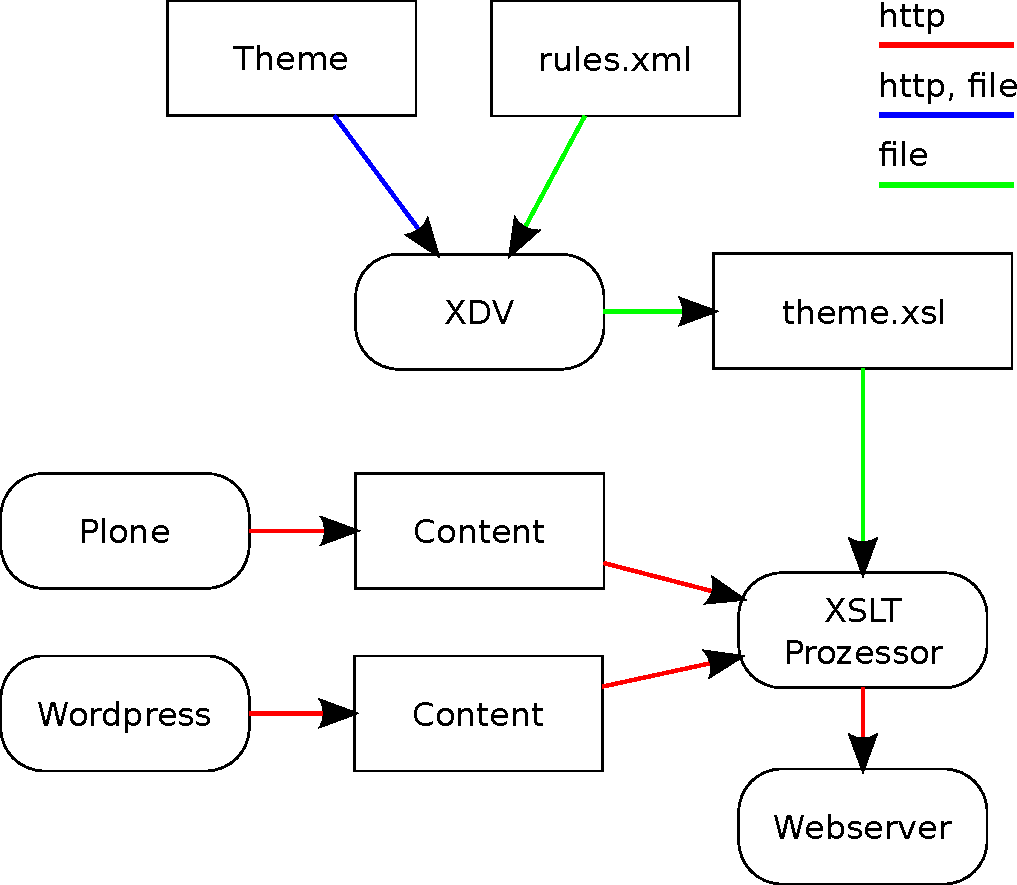
\includegraphics[scale=0.45]{resources/xdv-systemskizze}
}

\section{Case Study}
\subsection{Gruene Akademie}
\frame {
    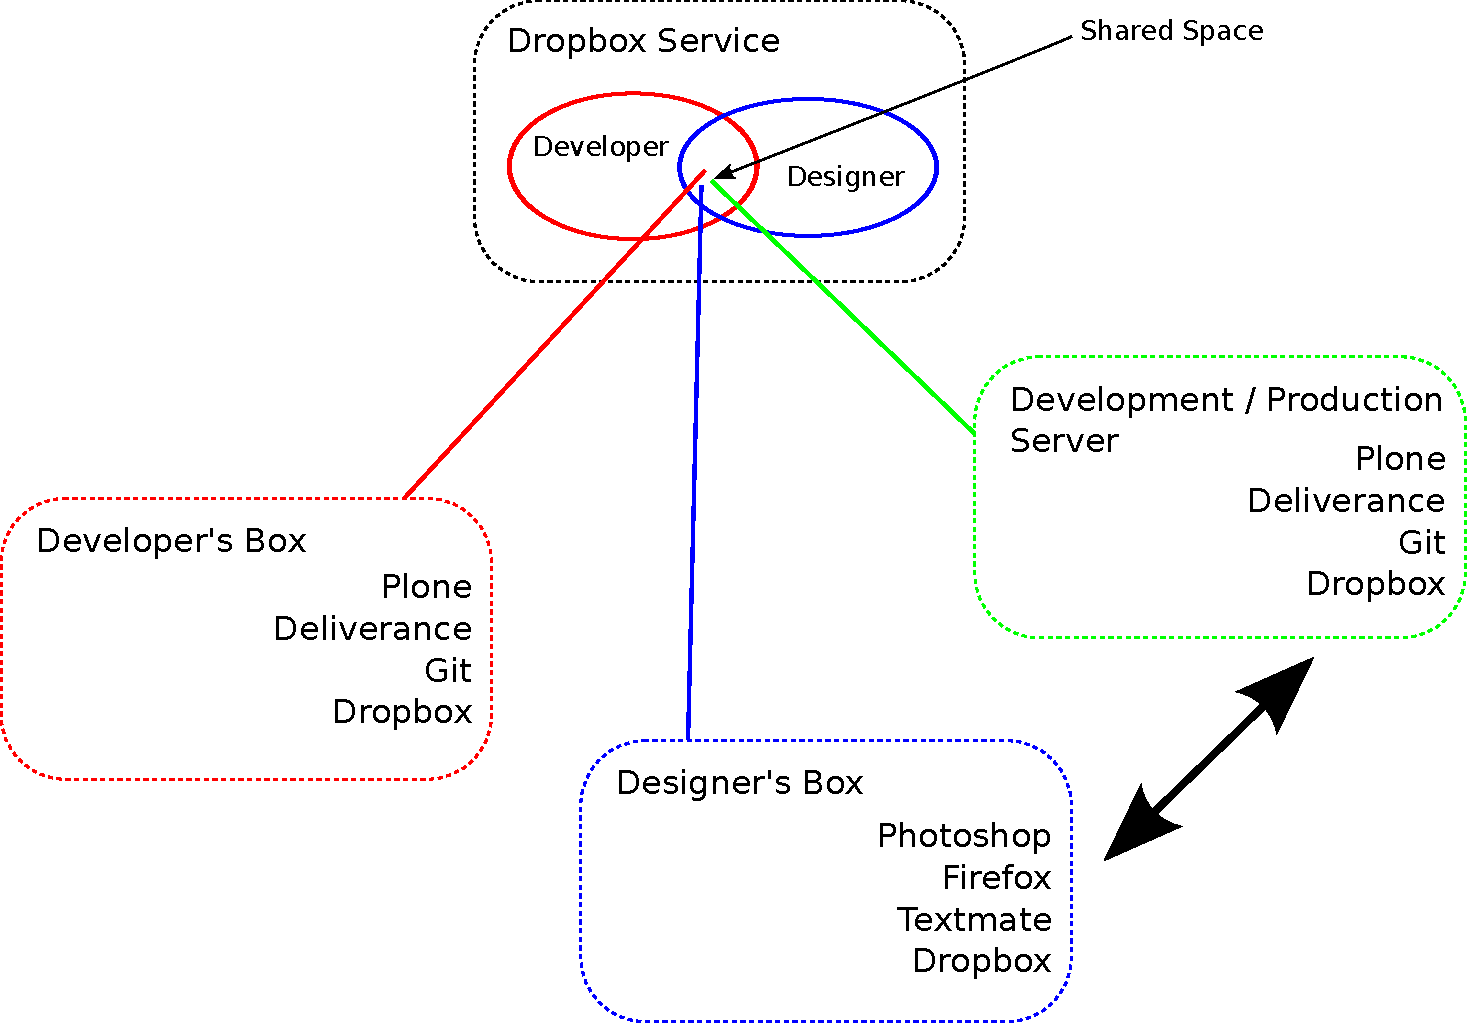
\includegraphics[scale=0.4]{resources/gruene-akademie-setup}
}
\frame {
    \begin{itemize}
        \item \url{http://gruene-akademie.at/}
        \item Automatisches Theme Update (5 Sekunden Delay)
        \item Bei Projektabschluss kann Dropbox Service wieder deaktiviert werden
    \end{itemize}
}


\section{Outro}
\subsection{Links}
\frame {
    \begin{itemize}
    \item Deliverance
        \begin{itemize}
        \item Info: \url{http://deliveranceproject.org/}
        \item PyPi: \url{http://pypi.python.org/pypi/Deliverance}
        \item Doku: \url{http://packages.python.org/Deliverance/}
        \item Code: \url{https://projects.openplans.org/deliverance/}
        \end{itemize}
    \item XDV
        \begin{itemize}
        \item PyPi: \url{http://pypi.python.org/pypi/xdv}
        \item XDV/Plone: \url{http://pypi.python.org/pypi/collective.xdv}
        \item Code: \url{http://codespeak.net/svn/z3/xdv/}
        \end{itemize}
    \item Mehr...
        \begin{itemize}
        \item Vortrag: \url{http://github.com/thet/dzug11.deliverance.vortrag}
        \item Buildout: \url{http://github.com/thet/dzug11.deliverance.buildout}
        \item Dropbox Integration: \url{http://bluedynamics.com/articles/johannes/drop-dead-dropbox-doings-with-deliverance}
        \end{itemize}
    \end{itemize}
}


\subsection{Dank an}
\frame {
    \frametitle{Dank an}
    \begin{itemize}
    \item Nate Aune
    \item Carsten Senger
    \item Rok Garbas
    \item Paul Everitt
    \item Deliverance \& XDV Team
    \end{itemize}
}



%\section{KAPITEL}
%\subsection{TITLE}
%\frame {
%    \frametitle{TITLE}
%    \begin{itemize}
%    \item
%    \end{itemize}
%}


%
